% Coupling in flow matching: independent (crossing, curved) vs reflow/OT (straight).
% Build:  pdflatex coupling.tex  &&  pdftocairo -svg coupling.pdf coupling.svg
\documentclass[border=6pt]{standalone}
\usepackage{tikz}
\usetikzlibrary{arrows.meta,positioning,fit,backgrounds}

\definecolor{noisec}{HTML}{6B7280}   % gray  - noise
\definecolor{catc}{HTML}{2563EB}     % blue  - cats mode
\definecolor{dogc}{HTML}{DC2626}     % red   - dogs mode
\definecolor{badc}{HTML}{B91C1C}     % crossing arrows
\definecolor{goodc}{HTML}{059669}    % straight arrows

\begin{document}
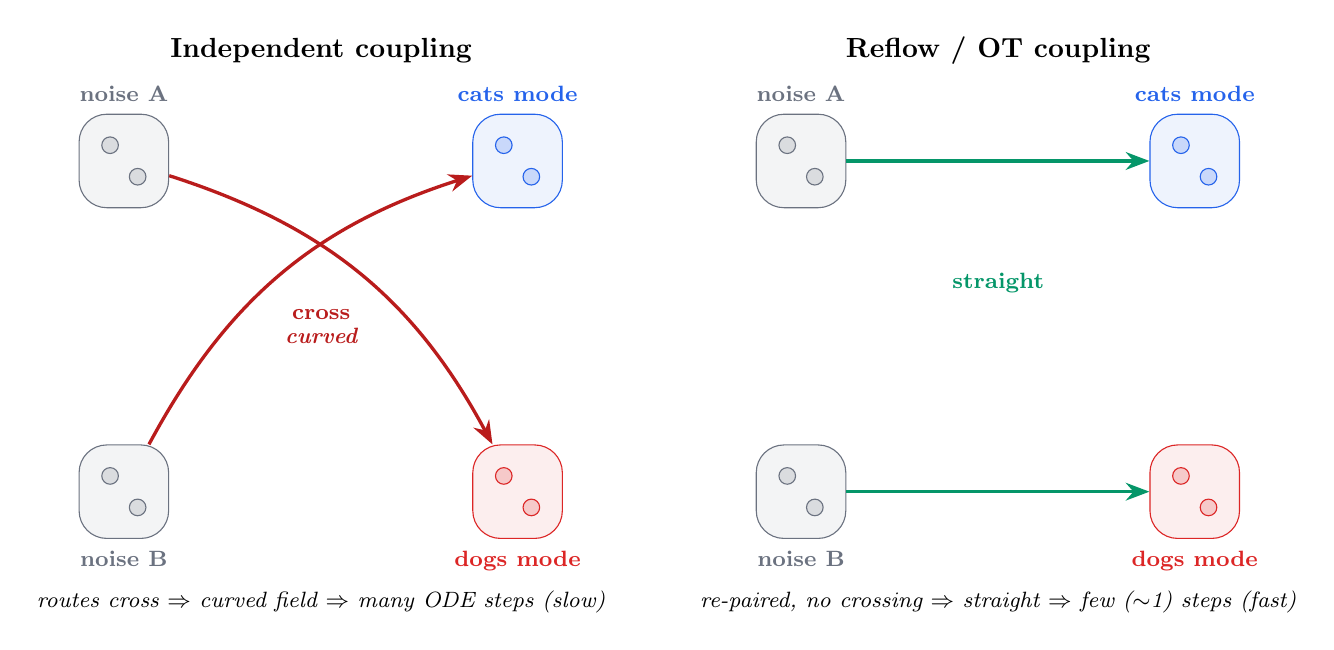
\begin{tikzpicture}[
    font=\small,
    dot/.style={circle,draw=#1,fill=#1!25,minimum size=6pt,inner sep=0pt},
    blob/.style={rounded corners=10pt,draw=#1,fill=#1!8,inner sep=8pt},
    lbl/.style={font=\footnotesize\bfseries},
  ]

% ======================= PANEL A: independent coupling =======================
\begin{scope}
  % noise source (one Gaussian, drawn as two sub-groups A/B)
  \node[dot=noisec] (a1) at (0,2.3) {};
  \node[dot=noisec] (a2) at (0.35,1.9) {};
  \node[dot=noisec] (b1) at (0,-1.9) {};
  \node[dot=noisec] (b2) at (0.35,-2.3) {};
  \begin{scope}[on background layer]
    \node[blob=noisec,fit=(a1)(a2)] (grpA) {};
    \node[blob=noisec,fit=(b1)(b2)] (grpB) {};
  \end{scope}
  \node[lbl,noisec,above=1pt of grpA] {noise A};
  \node[lbl,noisec,below=1pt of grpB] {noise B};

  % data targets (two modes)
  \node[dot=catc] (cat1) at (5,2.3) {};
  \node[dot=catc] (cat2) at (5.35,1.9) {};
  \node[dot=dogc] (dog1) at (5,-1.9) {};
  \node[dot=dogc] (dog2) at (5.35,-2.3) {};
  \begin{scope}[on background layer]
    \node[blob=catc,fit=(cat1)(cat2)] (grpCat) {};
    \node[blob=dogc,fit=(dog1)(dog2)] (grpDog) {};
  \end{scope}
  \node[lbl,catc,above=1pt of grpCat] {cats mode};
  \node[lbl,dogc,below=1pt of grpDog] {dogs mode};

  % crossing, curved arrows: A -> dogs, B -> cats
  \draw[-{Stealth[length=3mm]},badc,very thick,bend left=22]  (grpA) to (grpDog);
  \draw[-{Stealth[length=3mm]},badc,very thick,bend left=22]  (grpB) to (grpCat);

  \node[lbl,align=center] at (2.68,0) {\textcolor{badc}{cross}\\[-1pt]\textcolor{badc}{\itshape curved}};
  \node[font=\bfseries] at (2.68,3.5) {Independent coupling};
  \node[font=\itshape\footnotesize,align=center] at (2.68,-3.5)
    {routes cross $\Rightarrow$ curved field $\Rightarrow$ many ODE steps (slow)};
\end{scope}

% ======================= PANEL B: reflow / OT coupling =======================
\begin{scope}[xshift=8.6cm]
  \node[dot=noisec] (ra1) at (0,2.3) {};
  \node[dot=noisec] (ra2) at (0.35,1.9) {};
  \node[dot=noisec] (rb1) at (0,-1.9) {};
  \node[dot=noisec] (rb2) at (0.35,-2.3) {};
  \begin{scope}[on background layer]
    \node[blob=noisec,fit=(ra1)(ra2)] (rgrpA) {};
    \node[blob=noisec,fit=(rb1)(rb2)] (rgrpB) {};
  \end{scope}
  \node[lbl,noisec,above=1pt of rgrpA] {noise A};
  \node[lbl,noisec,below=1pt of rgrpB] {noise B};

  \node[dot=catc] (rcat1) at (5,2.3) {};
  \node[dot=catc] (rcat2) at (5.35,1.9) {};
  \node[dot=dogc] (rdog1) at (5,-1.9) {};
  \node[dot=dogc] (rdog2) at (5.35,-2.3) {};
  \begin{scope}[on background layer]
    \node[blob=catc,fit=(rcat1)(rcat2)] (rgrpCat) {};
    \node[blob=dogc,fit=(rdog1)(rdog2)] (rgrpDog) {};
  \end{scope}
  \node[lbl,catc,above=1pt of rgrpCat] {cats mode};
  \node[lbl,dogc,below=1pt of rgrpDog] {dogs mode};

  % straight arrows: A -> cats, B -> dogs
  \draw[-{Stealth[length=3mm]},goodc,very thick] (rgrpA) -- (rgrpCat);
  \draw[-{Stealth[length=3mm]},goodc,very thick] (rgrpB) -- (rgrpDog);

  \node[lbl,align=center] at (2.68,0.55) {\textcolor{goodc}{straight}};
  \node[font=\bfseries] at (2.68,3.5) {Reflow / OT coupling};
  \node[font=\itshape\footnotesize,align=center] at (2.68,-3.5)
    {re-paired, no crossing $\Rightarrow$ straight $\Rightarrow$ few ($\sim$1) steps (fast)};
\end{scope}

\end{tikzpicture}
\end{document}
